% -------------------------------------------------------------------
% Area de importação de pacotes do Latex
% -------------------------------------------------------------------

\documentclass[a4paper,12pt]{article}
\usepackage[english,brazilian]{babel}
\usepackage[utf8x]{inputenc}

\usepackage[a4paper,left=30mm,right=20mm,top=30mm,bottom=20mm,includehead,includefoot]{geometry}

\usepackage{setspace}
\onehalfspacing %% 1,5-spacing

\usepackage{graphicx}
\graphicspath{ {./imgs/} }

\usepackage{amsmath}

% -------------------------------------------------------------------
% -------------------------------------------------------------------
\begin{document}

\title{ \large \textbf{Atividade 1: Aplicações e propriedades probabilísticas}}
\date{\vspace{-5ex}}
\maketitle

\begin{flushright}
  { \bf Alan Utsuni Sabino }
\end{flushright}

\section{Bernoulli}

\paragraph{} Se aplica a situações em que as alternativas são
dicotômicas e podem ser representadas genericamente por resposta do
tipo {\it sucesso-fracasso}. Esses experimentos recebem o nome de {\it
  Ensaios de Bernoulli} e originam uma variável aleatória com
distribuição de Bernoulli que assume apenas dois valores: 1, se
ocorrer sucesso, e 0, se ocorrer fracasso.

%\[ \left \{
%  \begin{tabular}{c}
%      1, se ocorrer sucesso \\
%      0, se ocorrer fracasso
%  \end{tabular}
%\right.
%\]

A probabilidade de sucesso do evento de interesse pode ser
representada por {\it p}, $0<p<1$, e {\it 1-p} a probabilidade de
fracasso com sua função de probabilidade podendo ser representada pela
tabela:

\begin{center}
  \begin{tabular}{c|cc}
    $X$ & 1 & 0 \\
    \hline
    $P(X=x)$ & $p$ & $1-p$
  \end{tabular}
\end{center}

\setlength{\parindent}{0pt} {\bf Exemplo:} Um pacote de informações é
enviado pela internet ao receptor através de uma conexão, sendo {\it
  0.7} a probabilidade de que o pacote chegue corretamente ao
receptor. Uma representação gráfica da distribuição de Bernoulli é a
que segue:

\begin{figure}[h!]
  \begin{center}
    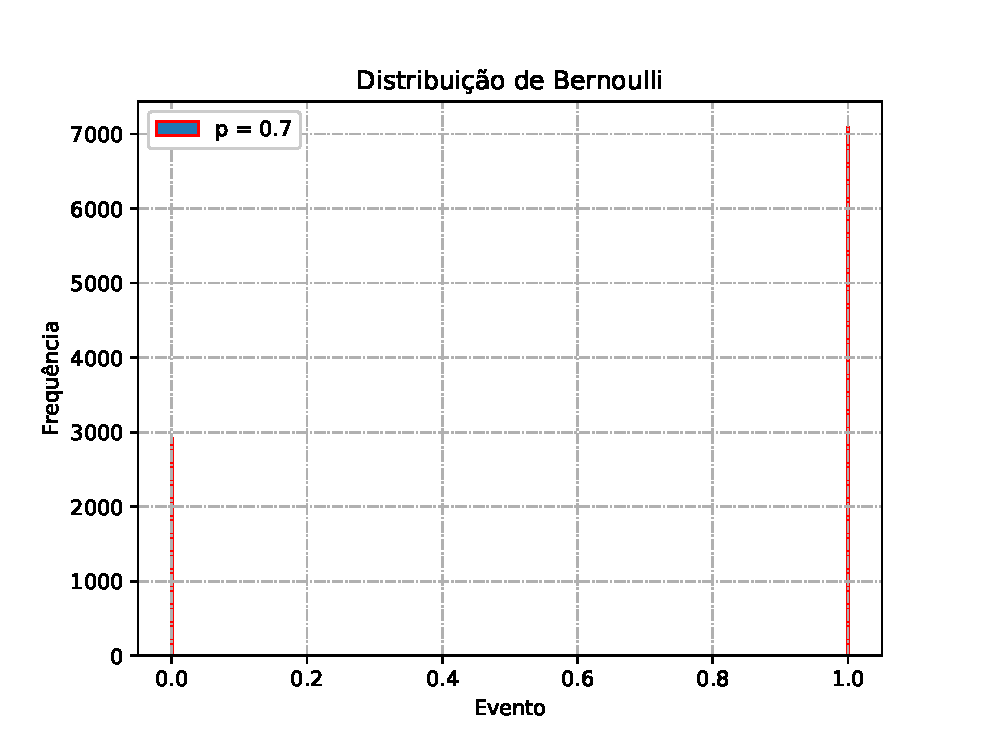
\includegraphics[scale=0.41]{bernoulli07.eps}
  \end{center}
\end{figure}

\section{Binomial}

\paragraph{} Considere {\it n} experimentos independentes
identicamente distribuídos, cada um com distribuição Bernoulli de
parâmetro {\it p} e a variável aleatória de interesse X corresponde ao número de
sucessos obtidos nestes {\it n} experimentos, então X é conhecida como
uma variável aleatória binomial de parâmetros {\it n} e {\it p}. Sua
função de probabilidade é dada por:

$$ P(X = k) = \binom{n}{k} p^k (1-p)^{n-k}$$

em que $ 0 \le k \le n $. \\

{\bf Exemplo:} {\it 10} pacotes de informação são enviados pela
internet ao receptor através de uma conexão. A probabilidade de cada
um dos pacotes chegar corretamente é igual a {\it 0.7}. Qual é a
probabilidade de que {\it 6} pacotes de informação enviados cheguem
corretamente ao receptor?

$$ P(X = 6) = \binom{10}{6} 0.7^6 (1-0.7)^{10-6} = 0,2$$

\begin{figure}[h!]
  \begin{center}
    \includegraphics[scale=0.41]{binomial1007.eps}
  \end{center}
\end{figure}

\section{Binomial negativa}

\paragraph{}
Aenean pellentesque id nisl pellentesque congue. Donec maximus dui vel
ullamcorper facilisis. Cras at suscipit est. Aenean ac velit
erat. Duis accumsan tincidunt felis, eu efficitur sapien. Phasellus
mattis tellus nunc, eu ullamcorper lorem faucibus sed. Vivamus
lobortis id enim hendrerit commodo. Fusce ac mattis elit. Orci varius
natoque penatibus et magnis dis parturient montes, nascetur ridiculus
mus. Pellentesque sit amet felis odio. Morbi hendrerit elit eget
venenatis viverra. Aliquam ut condimentum dolor. Curabitur eros risus,
efficitur ac libero et, dignissim rutrum turpis. Proin non blandit
tortor. Cras volutpat rhoncus ipsum, eu egestas est placerat at.

\section{Poisson}

\paragraph{}
Aenean pellentesque id nisl pellentesque congue. Donec maximus dui vel
ullamcorper facilisis. Cras at suscipit est. Aenean ac velit
erat. Duis accumsan tincidunt felis, eu efficitur sapien. Phasellus
mattis tellus nunc, eu ullamcorper lorem faucibus sed. Vivamus
lobortis id enim hendrerit commodo. Fusce ac mattis elit. Orci varius
natoque penatibus et magnis dis parturient montes, nascetur ridiculus
mus. Pellentesque sit amet felis odio. Morbi hendrerit elit eget
venenatis viverra. Aliquam ut condimentum dolor. Curabitur eros risus,
efficitur ac libero et, dignissim rutrum turpis. Proin non blandit
tortor. Cras volutpat rhoncus ipsum, eu egestas est placerat at.

\section{Geométrica}

\paragraph{}
Aenean pellentesque id nisl pellentesque congue. Donec maximus dui vel
ullamcorper facilisis. Cras at suscipit est. Aenean ac velit
erat. Duis accumsan tincidunt felis, eu efficitur sapien. Phasellus
mattis tellus nunc, eu ullamcorper lorem faucibus sed. Vivamus
lobortis id enim hendrerit commodo. Fusce ac mattis elit. Orci varius
natoque penatibus et magnis dis parturient montes, nascetur ridiculus
mus. Pellentesque sit amet felis odio. Morbi hendrerit elit eget
venenatis viverra. Aliquam ut condimentum dolor. Curabitur eros risus,
efficitur ac libero et, dignissim rutrum turpis. Proin non blandit
tortor. Cras volutpat rhoncus ipsum, eu egestas est placerat at.

\section{Hipergeométrica}

\paragraph{}
Aenean pellentesque id nisl pellentesque congue. Donec maximus dui vel
ullamcorper facilisis. Cras at suscipit est. Aenean ac velit
erat. Duis accumsan tincidunt felis, eu efficitur sapien. Phasellus
mattis tellus nunc, eu ullamcorper lorem faucibus sed. Vivamus
lobortis id enim hendrerit commodo. Fusce ac mattis elit. Orci varius
natoque penatibus et magnis dis parturient montes, nascetur ridiculus
mus. Pellentesque sit amet felis odio. Morbi hendrerit elit eget
venenatis viverra. Aliquam ut condimentum dolor. Curabitur eros risus,
efficitur ac libero et, dignissim rutrum turpis. Proin non blandit
tortor. Cras volutpat rhoncus ipsum, eu egestas est placerat at.

\end{document}

% Bernoulli
% http://www.de.ufpb.br/~tarciana/MPIE/Aula7.pdf
% https://www.ime.usp.br/~yambar/MAE116-Quimica/Aula%205%20Distribui%E7%E3o%20Binomial/Aula%205%20-%20Distribui%E7%E3o%20Binomial.pdf
% https://edisciplinas.usp.br/pluginfile.php/1804481/mod_resource/content/1/aula3-2016.pdf